\section{Pager}
Un vantaggio della memoria virtuale è quello di poter caricare in modo dinamico i frame fisici dalla memoria secondaria. Il modulo del sistema operativo che si occupa della paginazione su richiesta è il \textit{pager}.

\spacer
Il termine \textit{swapping} indica l'atto di inserire o rimuovere delle pagine dalla memoria.
Quando una pagina viene rimossa dalla memoria essa viene riportata in un dispositivo di memroia secondaria, all'interno di un file (Windows) o una partizione (linux)

\spacer
Spesso si utilizza uno swapper pigro, che carica le pagine in RAM solo quando esse vengono richieste.

\begin{note}
    Inoltre spesso si utilizza una partizione di swap sulla memoria secondaria per ampliare ulteriormente le dimensioni della memoria principale, essa permette di ottenere delle prestazioni migliori in quanto non incorre nella frammentazione dei dischi.
\end{note}

Per sapere quali pagine si trovano già in memoria e quali invece devono essere caricate il pager utilizza una tabella delle pagine, essa associa la memoria logica a quella fisica. Inoltre comprende un bit di validità che specifica se il frame si trova in memoria o meno.

\begin{figure}[H]
    \centering
    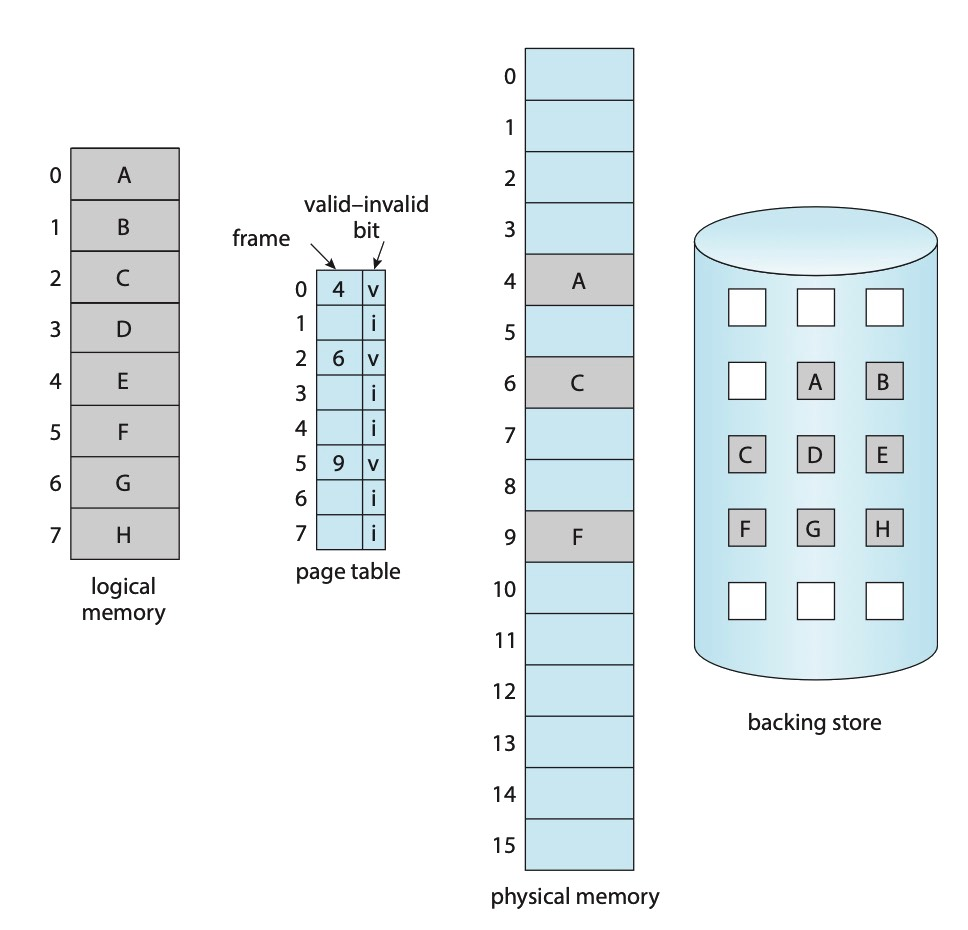
\includegraphics[width=0.45\linewidth]{assets/tabella-pagine.jpg}
\end{figure}

\subsection{Page Fault}

Quando il programma richiede un indirizzo appartenente ad una pagina non caricata in memoria causa una trap al sistema operativo, una \textit{page fault}.

A questo punto il sistema operativo consulta una sua tabella delle pagine e invia al programma un abort se l'indirizzo non è valido.

Se viene trovata la pagina nella memoria secondaria allora essa viene caricata nella RAM e l'esecuzione del programma può riprendere.

\begin{figure}[H]
    \centering
    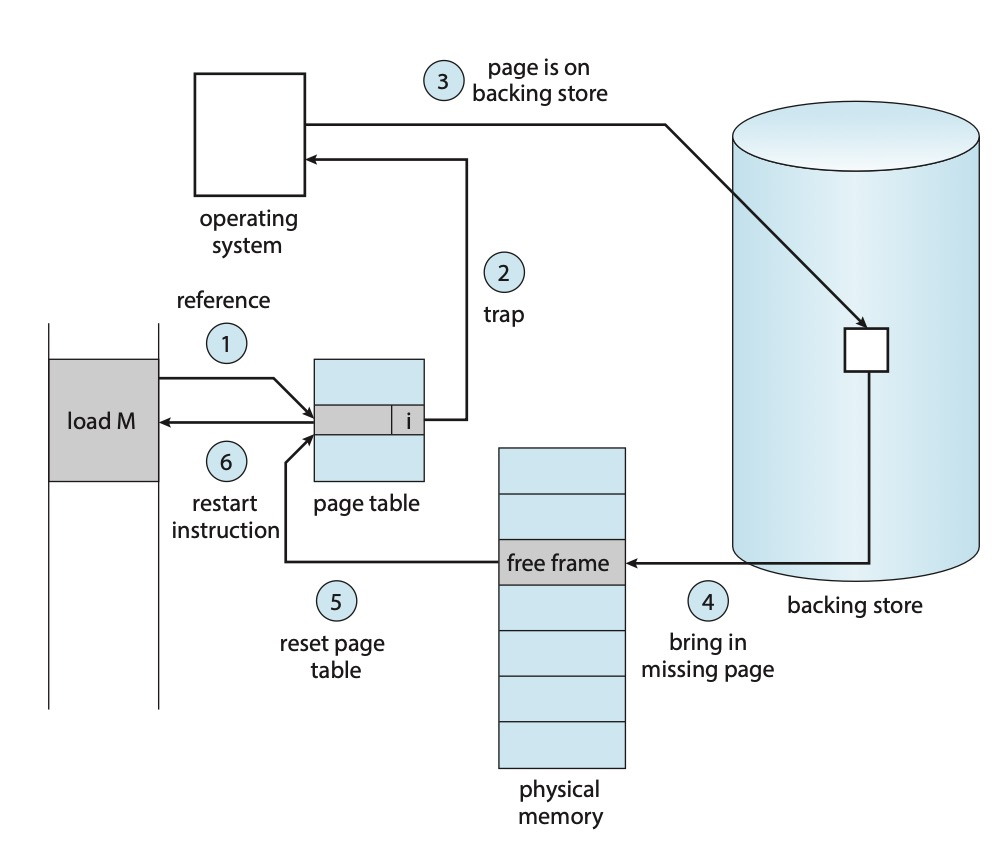
\includegraphics[width=0.5\linewidth]{assets/gestione-page-fault.jpg}
\end{figure}

Se non sono disponibili dei frame liberi nella memoria principale sarà necessario rimuovere prima una pagina secondo un algoritmo di selezione.
Si ricerca un algoritmo che riduca al minimo il numero di page fault in quanto esse sono un fattore importante sulle prestazioni del sistema.

\spacer
Viene impiegato un bit di modifica, o \textit{dirty bit}, per ridurre l'overhead dei trasferimenti di pagine. Solo le pagine modificate vengono riscritte al disco, le altre possono essere semplicemente sovrascritte.

\subsubsection{Prestazioni}
Il tempo effettivo di accesso alla memoria (EAT) si può calcolare nel seguente modo:
$$EAT = (1 - p)\cdot \text{accesso alla memoria} + p \cdot \text{overhead page fault}$$

Dove p è la probabilità di ottenere un page fault.

\spacer
Assumendo dei valori realistici, il tempo di acccesso alla memoria è di circa 200ns, mentre l'overhead per un page fault 8ms.

Sotto queste ipotesi se si ha un page fault ogni 1000 accessi l'accesso alla memoria viene mediamente rallentato di un fattore di 40.

Per ottenere un fattore di rallentamento accettabile (<0.1) è necessario arrivare ad un page fault ogni 400,000 richieste.

\subsection{Prepaging}
Per ridurre il gran numero di page fault che avvengono all'avvio del processo si può utilizzare il prepaging, ovvero si possono copiare un certo numero di pagine in memoria prima dell'esecuzione del programma.

\spacer
Ad esempio, se un programma è stato sospeso per una richiesta I/O, quando esso riprende l'esecuzione è possibile riportare in memoria il suo ultimo working set.

\spacer
È importante bilanciare le prestazioni di questa operazione ed assicurarsi che il vantaggio in riduzione di page fault sia superiore al costo di prepaging.

\subsection{Algoritmi di Paging}
Il paging richiede diversi algoritmi per un funzionamento corretto, in particolare sono necessari per l'allocazione dei frame e per la sostituzione delle pagine.

\begin{note}
    Alcune pagine devono rimanere bloccate (pinned) in memoria, non possono essere selezionate come vittime dagli algoritmi.
\end{note}

Gli algoritmi vengono valutati su una particolare stringa di riferimenti in memoria, ovvero 7 0 1 2 0 3 0 4 2 3 0 3 0 3 2 1 2 0 1 7 0 1.

\subsubsection{Algoritmo Ottimo}
L'algoritmo ideale è quello che rimuove la pagina che non verrà utilizzata per il periodo di tempo più lungo, in questo caso sulla stringa l'algoritmo genera 9 page fault.

Tuttavia questo non è possibile saperlo senza conoscere il futuro, cosa che il sistema non è ovviamente in grado di fare.

\subsubsection{FIFO}
L'algoritmo più semplice è forse quello FIFO, possiamo creare una coda con tutte le pagine di memoria fisica e sostituendo la prima entrata.

\begin{figure}[H]
    \centering
    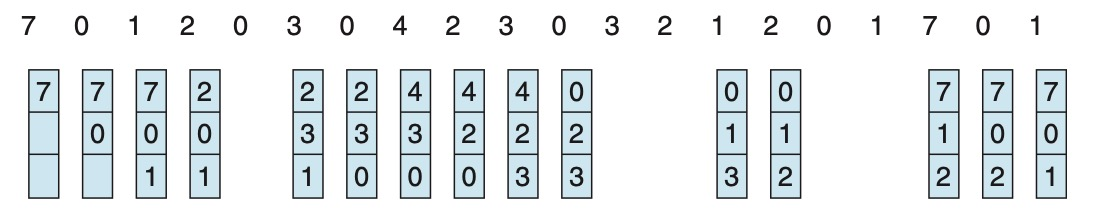
\includegraphics[width=0.5\linewidth]{assets/FIFO-paging-ex.jpg}
    \caption{Example when usign a 3 frame memory}
\end{figure}

\begin{note}
    Non sempre aumentare le dimensioni della memoria porta ad una riduzione del numero di page fault, questo fatto è noto come \textit{Anomalia di Belady}.

    In particolare usando una coda FIFO con string dei riferimenti 1 2 3 4 1 2 5 1 2 3 4 5
    \begin{figure}[H]
        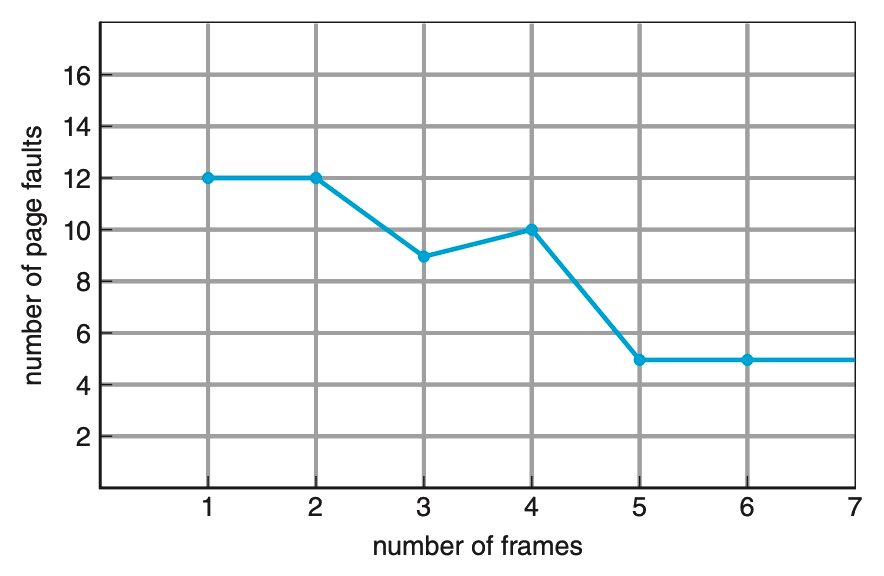
\includegraphics[width=0.4\linewidth]{assets/anomalia-belady.png}
    \end{figure}
\end{note}

\subsubsection{LRU}
L'algoritmo rimpiazza la pagina che non è stata utilizzata per più tempo, provando a prevedere il futuro conoscendo il passato.

Questo algoritmo genera 12 page fault sulla stringa di riferimento.

\spacer
LRU viene considerato un buon algoritmo per questa applicazione, tuttavia risulta esserne difficile l'implementazione. Ci sono diverse soluzioni per l'implementazione, ma tutte richiedono dell'hardware dedicato per renderle praticabili.

\subsubsection{LFU}
Least Frequently Used, si rimpiazza la pagina meno utilizzata.

\subsubsection{MFU}
Most Frequently Used, si basa sull'idea che la pagina utilizzata più di recente non deve essere ricopiata in memoria per essere rimpiazzata.

\subsubsection{Seconda Chance}
L'algoritmo si basa su un algoritmo FIFO, ma viene aggiunto un bit di riferimento ad ogni pagina.

Il bit di riferimento di tutte le pagine viene inizialmente impostato a 0, quando vengono utilizzate viene impostato ad 1.

\spacer
Quando è necessario sostituire una pagina si cerca nella coda FIFO, se si incontra uno 0 quella pagina verrà rimossa. Altrimenti se si incontra un 1 si dà alla pagina una seconda chance, impostando il bit a 0 e spostandosi oltre.

\begin{figure}[H]
    \centering
    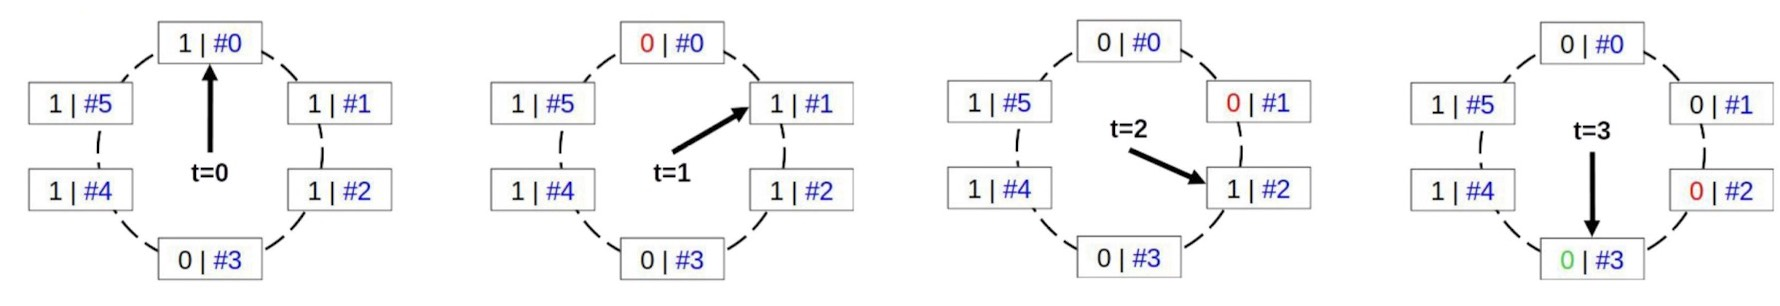
\includegraphics[width=0.9\linewidth]{assets/algoritmo-seconda-chance.jpg}
\end{figure}

L'algoritmo può essere migliorato tenendo conto anche del bit di modifica, si consideri la coppia (bit di riferimento, bit di modifica).

La pagina migliore è quella con valore (0, 0), seguita da (0, 1) che ha il difetto di dover essere salvata sulla memoria secondaria.

\subsubsection{Pool di Frame Liberi}
L'algoritmo richiede che venga sempre mantenuto un certo numero di frame liberi in memoria. Questi vengono utilizzati da buffer, dopo la selezione del frame vittima il nuovo frame viene scritto in uno dei frame liberi e infine il frame vittima viene copiato in memoria secondaria.

\spacer
Un'altra ottimizzazione disponibile è quella di controllare la memoria secondaria e quando esso è inattivo utilizzarlo per copiare dei frame modificati, resettando il loro bit di modifica.

\subsection{Allocazione dei Frame}
Il numero minimo di pagine che viene allocato ad un processo è deciso dall'architettura, mentre il massimo è dettato dalla dimensione della memoria primaria.

\subsubsection*{Allocazione Uniforme}
Semplicemente divide lo spazio della memoria per i programmi in esecuzione, quindi se si hanno 100 frame e 5 processi ognuno otterrà 20 frame.

\subsubsection*{Allocazione Proporzionale}
Uno schema di allocazione proporzionale alla dimensione del processo, un processo con più frame riceverà più risorse.

\subsubsection*{Allocazione con Priorità}
Si impiega uno schema basato sulla priorità, questa stessa priorità viene utilizzata anche per la scelta dei frame da rimuovere, un processo a priorità maggiore rimuoverà frame di processi a priorità inferiore.

\subsubsection*{Allocazione locale e globale}
L'allocazione globale permette ai processi di prendere frame da qualsiasi altro processo in esecuzione, quella locale invece limita le scelte ai frame che appartengono già al processo.

\spacer
Nei sistemi moderni si preferisce l'allocazione globale in quanto spesso garantisce un numero minore di page fault.

\subsection{Mappatura di File}
La mappatura di file in memoria permette l'accesso in modo completamente simile a quanto si fa per qualsiasi altro dato, l'accesso iniziale avviene tramite un page fault grazie al quale viene copiata una pagina di dati alla memoria principale.

\spacer
Questo permette anche di condividere il file tra più programmi in modo semplice dato che si trova in memoria virtuale.

Purtroppo ci sono anche degli svantaggi, legati principalmente a mantenere l'integrità del file anche in presenza di concorrenza.
\spacer
Il file viene aggiornato effettivamente in memoria solo alla chiusura o quando il pager decide di resettare il bit di modifica.

\spacer
Tutti i moderni sistemi operativi supportano la mappatura di file in memoria principale, spesso tramite una chiamata di sistema (\texttt{mmap()}).
Alcuni sistemi utilizzano la mappatura di default, come Solaris, rimuovendo così l'overhead causato dalla system call.

\subsubsection{Mappatura dell'I/O}
È possibile condividere informazioni tra processo e dispositivo I/O grazie alla mappatura in memoria, ad esempio un processo può scrivere su degli indirizzi di memoria, dai quali la scheda video prenderà i dati da mostrare all'utente.

\subsubsection{Copy On Write}
Le pagine di memoria vengono condivise tra due o più processi, quando uno vuole scrivere su una pagina la copia prima in una nuova locazione di memoria e poi la modifica.

\begin{figure}[H]
    \centering
    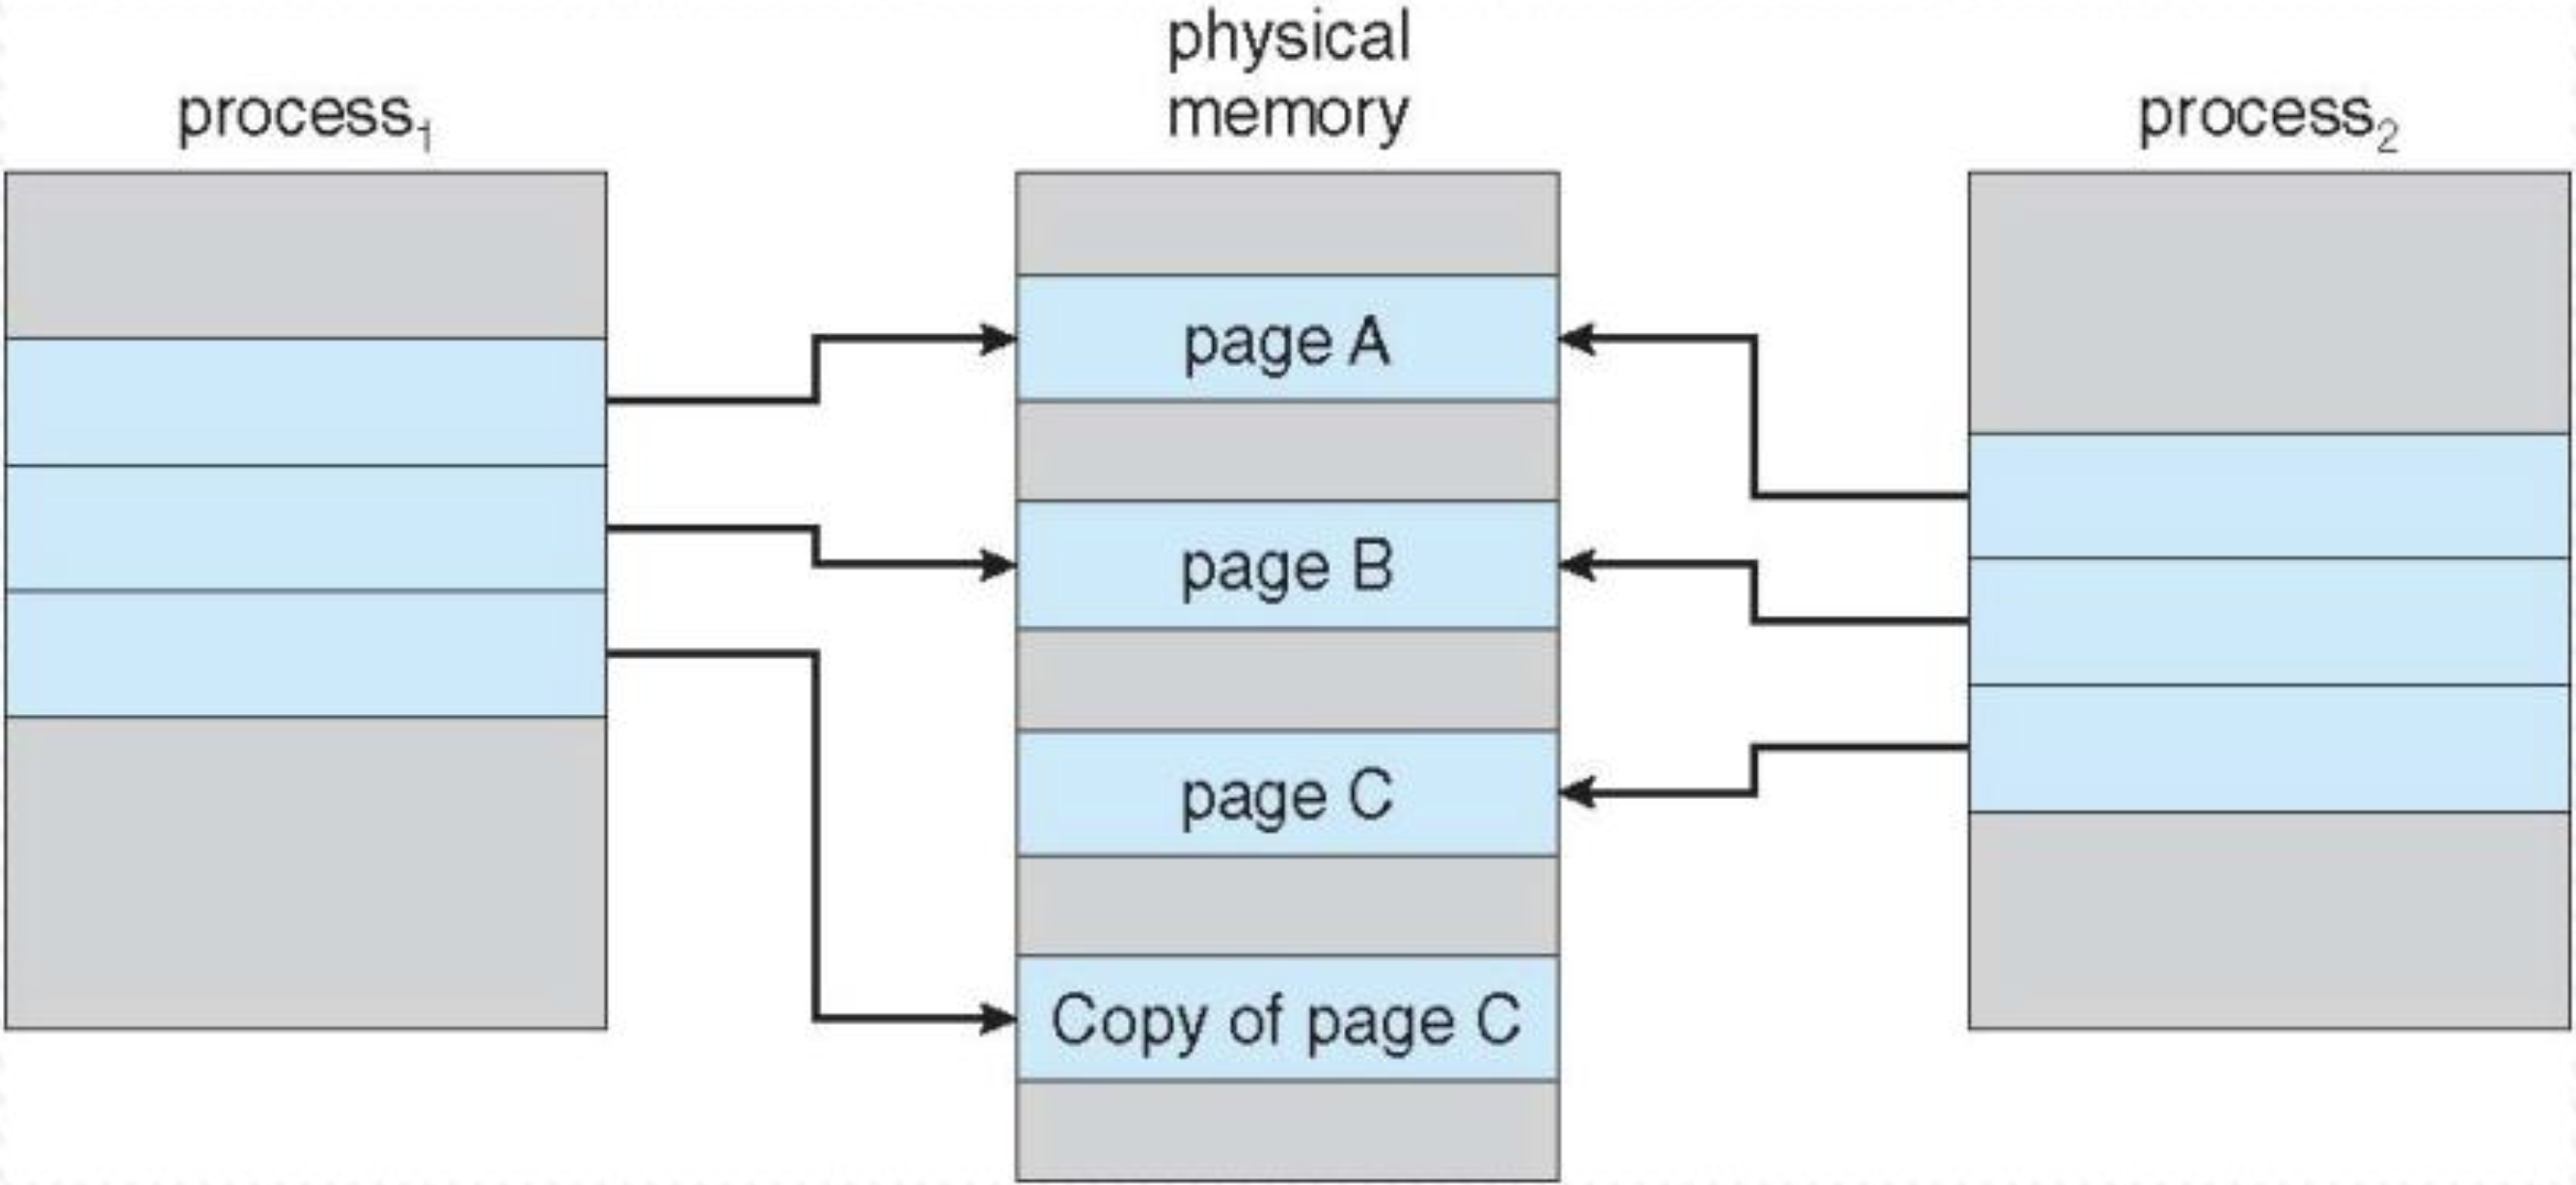
\includegraphics[width=0.5\linewidth]{assets/copy-on-write.png}
\end{figure}
